\section{Data Pre-processing}
\subsection{Load Data}
\begin{lstlisting}[language=R]
    # Importing data 
    intel_cpu <- read.csv ("~/Downloads/archive/Intel_CPUs.csv")
\end{lstlisting}

This line of R code is used to import a dataset from a Comma-Separated Values (CSV) file into the R environment.
The \texttt{read.csv()} function is a built-in function in R that reads a CSV file and creates a data frame object from its contents. A data frame is a two-dimensional tabular data structure in \texttt{R}, where each column represents a variable, and each row represents an observation.\\

In this specific code:
"\textbf{$\sim$/Downloads/archive/Intel\_CPUs.csv}" is the file path that specifies the location and name of the CSV file to be imported, \texttt{intel\_cpu} is the name assigned to the data frame object that will store the imported data.\\

After executing this line of code, the contents of the "\textbf{Intel\_CPUs.csv}" file will be read and stored in the \texttt{intel\_cpu} data frame within the \texttt{R} environment. The data frame will have the same structure as the CSV file, with columns representing variables and rows representing observations.

\subsection{Explore Data}
\begin{lstlisting}[language=R]
    # The head () function is used to preview the first 
    # few rows of the data frame
    head (intel_cpu)
\end{lstlisting}

This line calls the \texttt{head()} function and passes the \texttt{intel\_cpu} data frame as an argument. By default, the \texttt{head()} function prints the first \textit{six} rows of the given data frame or matrix.\\

The \texttt{head()} function is a valuable tool for data exploration and validation, especially when working with large datasets. By previewing the initial rows, you can quickly assess the structure of the data, check the column names, and ensure that the data has been imported correctly.\\

Inspecting the first few rows can reveal potential issues or anomalies in the data, such as missing values, incorrect data types, or unexpected values. It also provides an initial glimpse into the content and format of the data, which can inform subsequent data cleaning, transformation, or analysis steps

\begin{figure}[H]
    \centering
    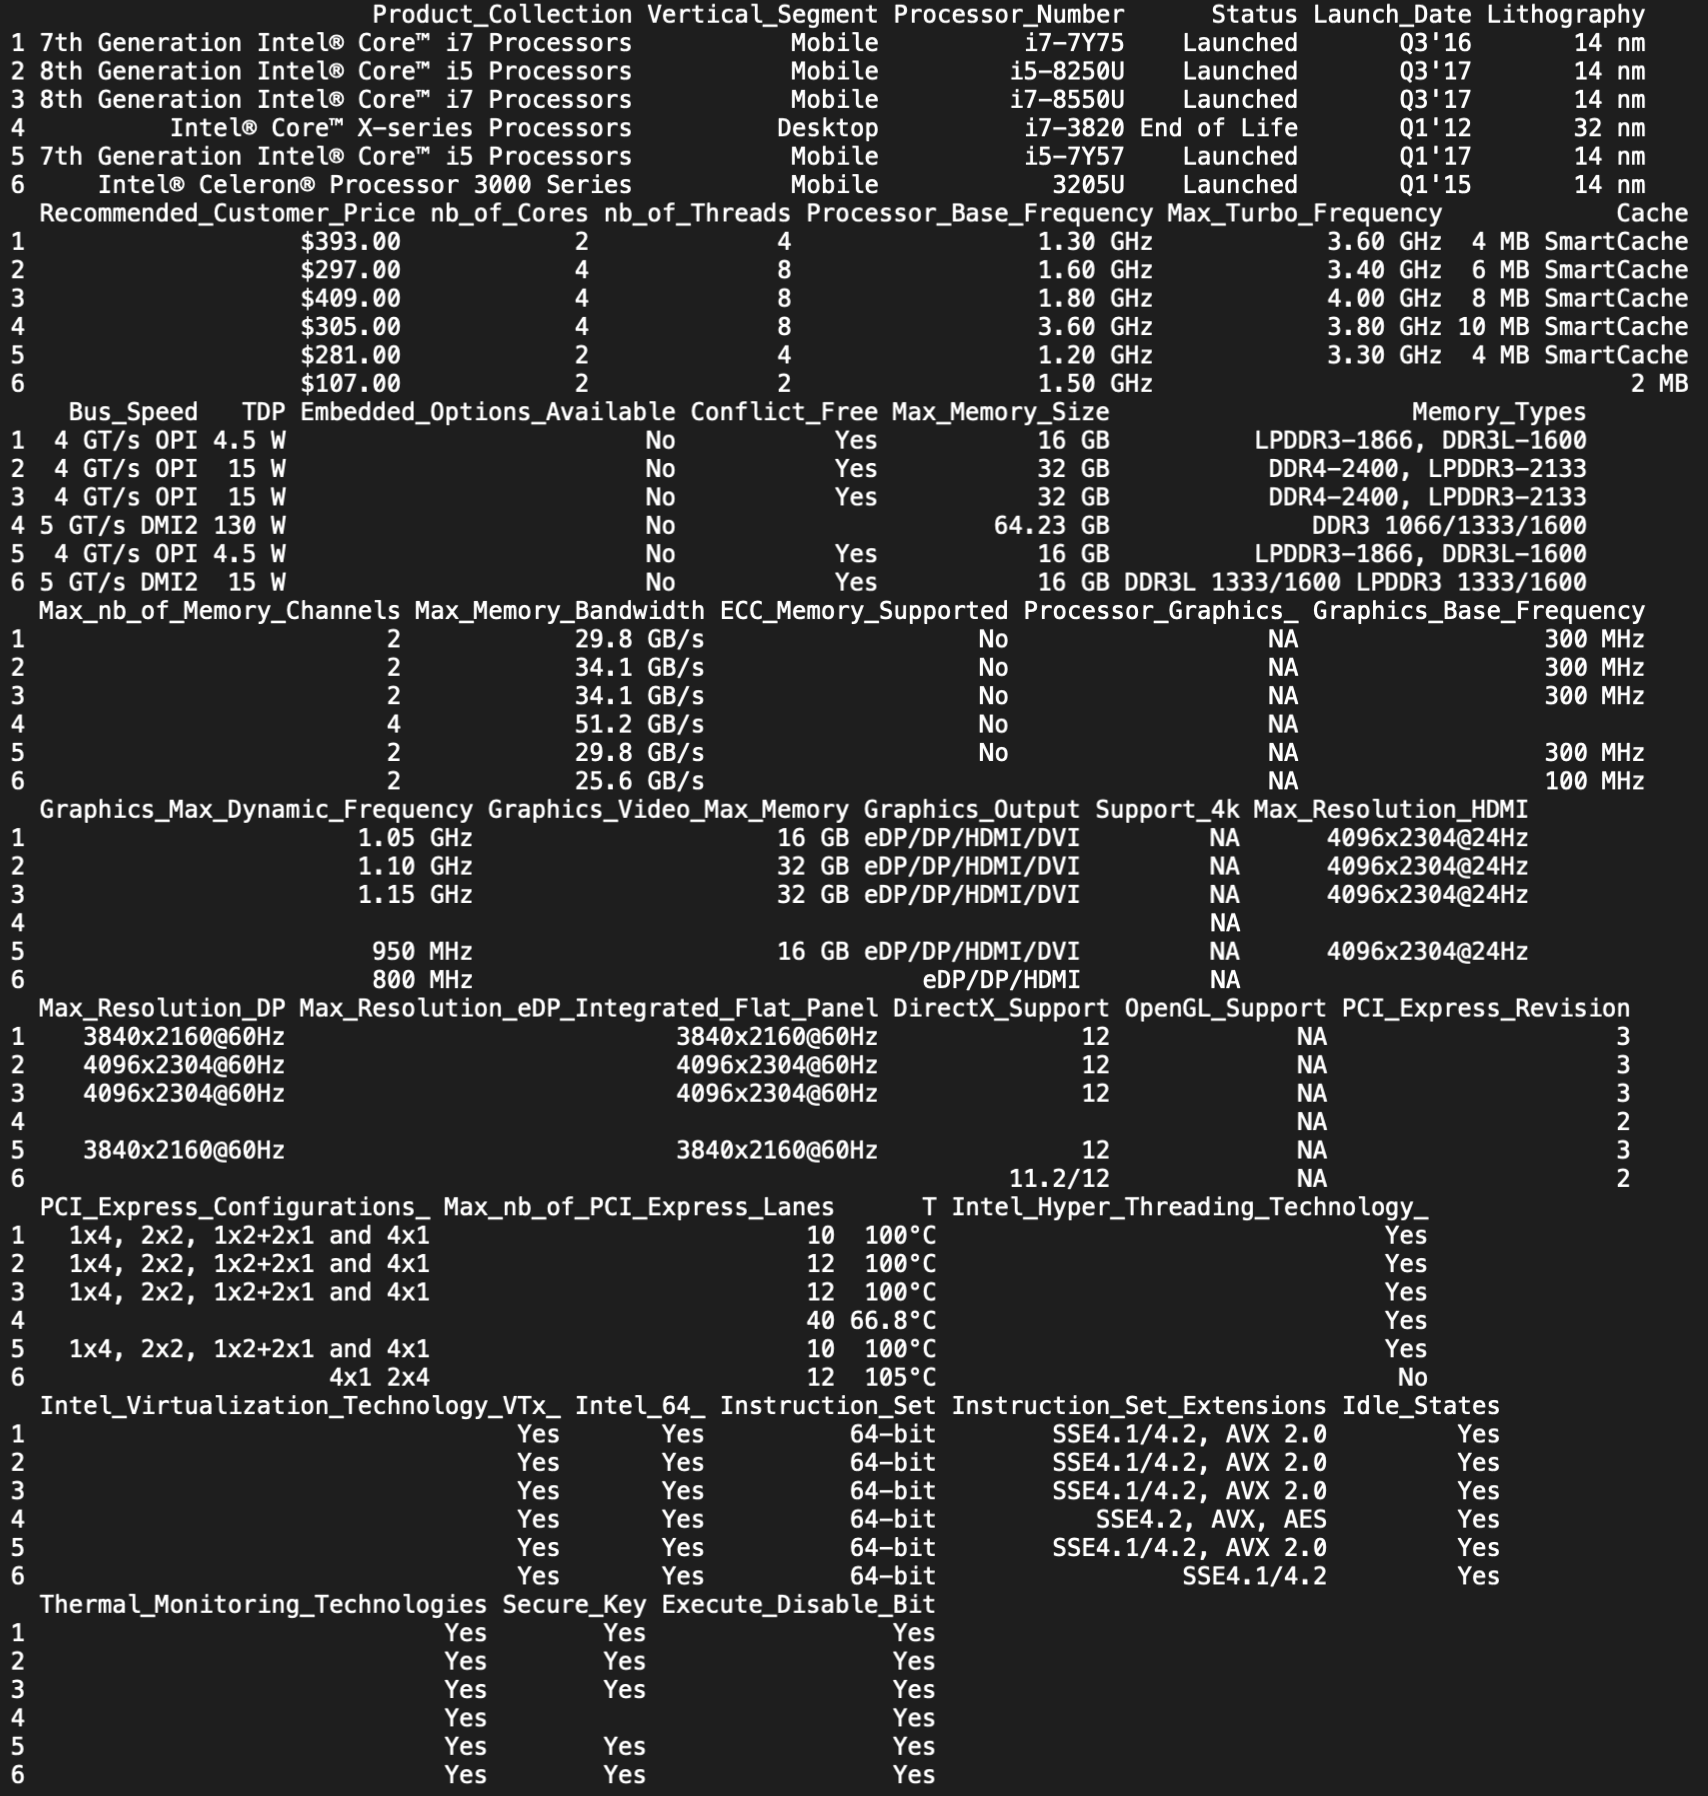
\includegraphics[width=14cm]{graphics/head.png}
    \caption*{Console output of \texttt{head(intel\_cpu)}}
\end{figure}

By executing \texttt{head(intel\_cpu)}, the output will display the first \textit{six} rows of the \texttt{intel\_cpu} data frame, allowing you to visually inspect the data and make informed decisions about the next steps in the data analysis workflow.

\newpage

\begin{lstlisting}[language=R]
    # Summary statistics
    summary (intel_cpu)
\end{lstlisting}

This code snippet is used to obtain summary statistics for the dataset stored in \texttt{intel\_cpu}.\\

The \texttt{summary ()} function in \texttt{R} is a versatile tool that provides a consise summary of the data, depending on the type of input it receives.

\begin{figure}[H]
    \centering
    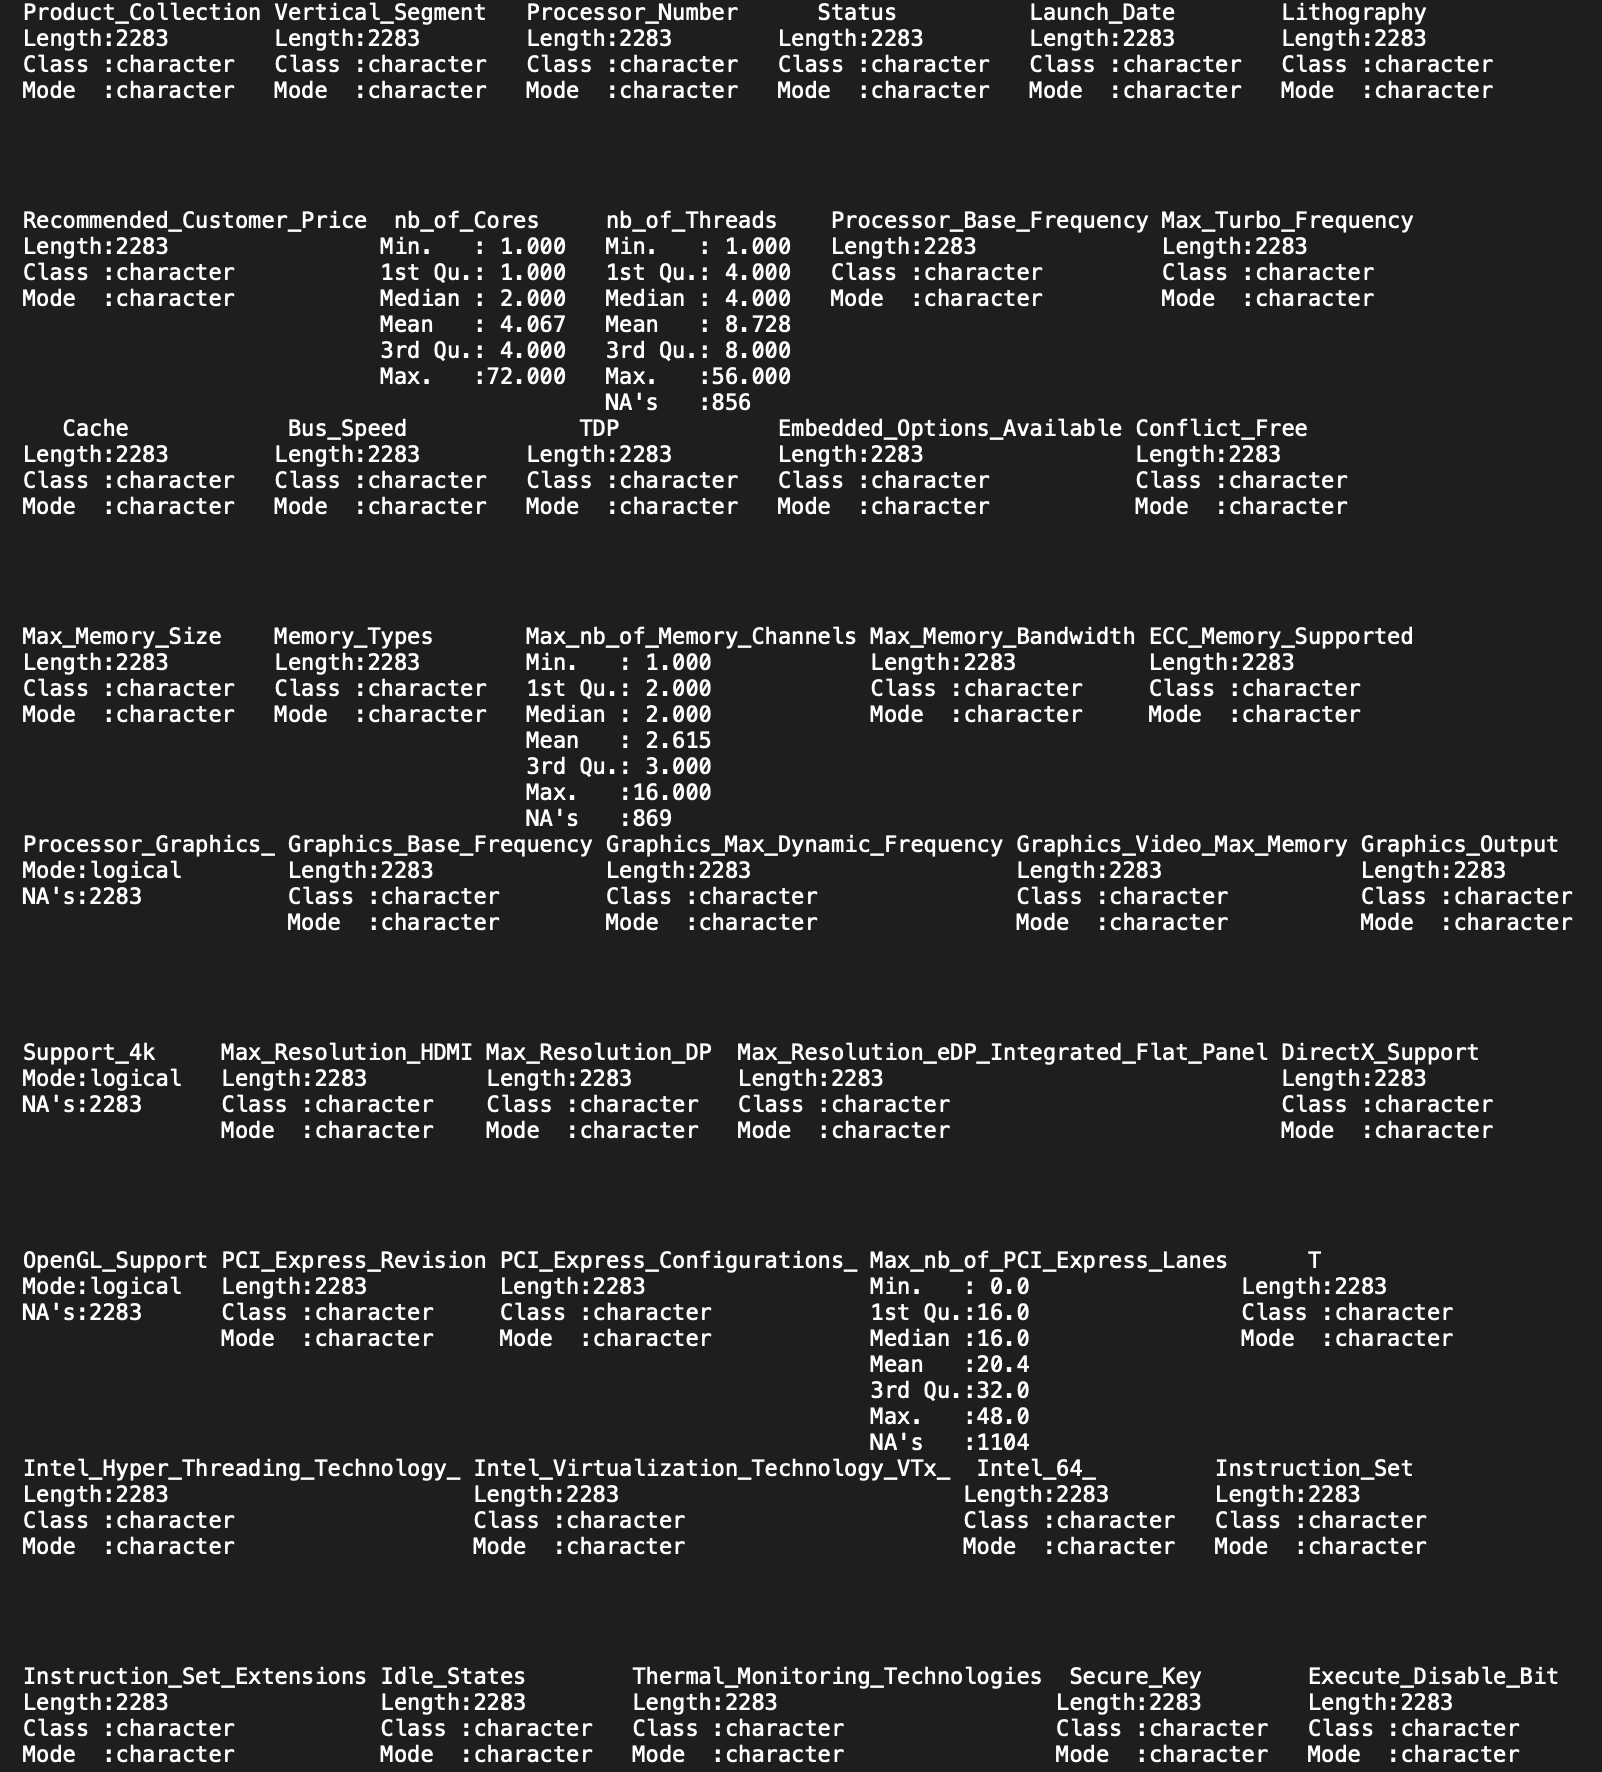
\includegraphics[width=14cm]{graphics/summary.png}
    \caption*{Console output of \texttt{summary(intel\_cpu)}}
\end{figure}

\subsection{Handle Missing Values}

\subsection{Handle Outliers}

\subsection{Feature Scaling/Normalization}

\newpage